\documentclass{article}

\usepackage[final]{style}
\usepackage[utf8]{inputenc} % allow utf-8 input
\usepackage[T1]{fontenc}    % use 8-bit T1 fonts
\usepackage{hyperref}       % hyperlinks
\usepackage{url}            % simple URL typesetting
\usepackage{booktabs}       % professional-quality tables
\usepackage{amsfonts}       % blackboard math symbols
\usepackage{nicefrac}       % compact symbols for 1/2, etc.
\usepackage{microtype}      % microtypography
\usepackage{verbatim}
\usepackage{graphicx}       % for figures

\usepackage{caption}
\usepackage{graphicx, subfig}

\usepackage{amsmath,bm}

\usepackage{mathrsfs}
\usepackage{amssymb}

% Self-defined macros
\newcommand{\matr}[1]{\mathbf{#1}}
\newcommand{\proba}[1]{\mathsf{P}(#1)}
\newcommand{\expect}[1]{\mathsf{E}[#1]}
\newcommand{\var}[1]{\mathsf{Var}(#1)}
\newcommand\defeq{\stackrel{\text{!}}{=}}

\title{Exercise 05 of Machine Learning [IN 2064]}

\author{
  Name: Yiman Li \\
  \textbf{Matr-Nr: 03724352} \\
  cooperate with Kejia Chen(03729686)\\
}

\begin{document}

\maketitle

\section*{Problem 1}
a) We can try to calculate the distribution of the posterior distribution as below:
\begin{eqnarray}
p(y=1|x)= \frac{p(x|y=1)p(y=1)}{p(x|y=1)\cdot p(y=1)+p(x|y=0)\cdot p(y=0)}= \frac{\lambda_1e^{-\lambda_1x}}{\lambda_1e^{-\lambda_1x}+\lambda_0e^{\lambda_0}} = \theta\\
p(y=0|x)= \frac{p(x|y=0)p(y=0)}{p(x|y=1)\cdot p(y=1)+p(x|y=0)\cdot p(y=0)}= \frac{\lambda_0e^{-\lambda_0x}}{\lambda_1e^{-\lambda_1x}+\lambda_0e^{\lambda_0}} = 1-\theta
\end{eqnarray}
So we can write that
\begin{equation}
p(y|x) = \theta^{\prod(y=1)}(1-\theta)^{\prod(y=0)}
\end{equation}
Which is a Bernoulli distribution.\\
b) Now that $x$ are classified as class 1, which means
\begin{equation}
p(y=1|x) > p(y=0|x)
\end{equation}
So we have
\begin{eqnarray}
\lambda_1e^{-\lambda_1x} > \lambda_0e^{-\lambda_0x}\\
\frac{\lambda_1}{\lambda_0} > e^{(\lambda_1-\lambda_0)x}\\
\mathrm{ln}\frac{\lambda_1}{\lambda_0} > (\lambda_1-\lambda_0)x
\end{eqnarray}
\begin{itemize}
	\item When $\lambda_1>\lambda_0$, $x < \frac{\mathrm{ln}\lambda_1 - \mathrm{ln}\lambda_0}{\lambda_1-\lambda_0}$

	\item When $\lambda_1<\lambda_0$, $x > \frac{\mathrm{ln}\lambda_1 - \mathrm{ln}\lambda_0}{\lambda_1-\lambda_0}$
\end{itemize}



\section*{Problem 2}
According to the Book of Bishop \cite{bishop2007}, the maximum likelihood solution lack robustness to outliers. Namely, maximum likelihood estimation may often lead to overfitting for data sets that are linearly separable. This arises because the maximum likelihood solution occurs when the hyperplane corresponding to $\sigma=0.5$, equivalent to $\bm{w}^T\bm{\phi} = 0$, separates the two classes and the magnitude of $\bm{w}$ goes to infinity.\\
Considering the picture shown in  Figure \ref{Fig.Bishop}:
\begin{figure}
	\centering
	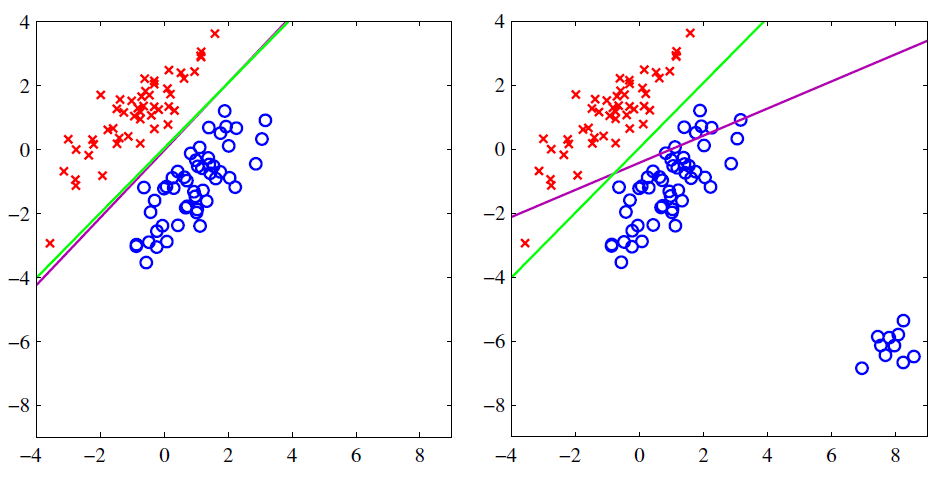
\includegraphics[scale=0.5]{MLEvsLRM.png}
	\caption{Contrast between least squares and logistic regression model}
	\label{Fig.Bishop}		
\end{figure}
there are two classes of data, denoted bu red crosses and blue circles, together with the decision boundary found by least squares(magenta curve) and also by logistic regression model(green curve). We can see that the additional data points in the right figure produce a significant change in the location of the decision boundary, even though these points would be correctly classified by the original decision boundary in the left figure.\\
We can control this by penalizing large weights, just as what we do in linear regression:
\begin{equation}
E(\bm{w}) = -\mathrm{ln}\ p(\bm{y}|\bm{w, X}) + \lambda||\bm{w}||_q^2
\end{equation}
Like before, for $q=2$ this corresponds to MAP estimation with a Gaussian prior on $\bm{w}$.



\section*{Problem 3}
For the case of $K>2$ classes, we have
\begin{equation}
\begin{aligned}
p(\mathcal{C}_k|x)
&= \frac{p(\bm{x}|\mathcal{C}_k)p(\mathcal{C}_k)}{\sum_{j}p(\bm{x}|\mathcal{C}_j)p(\mathcal{C}_j)}\\
&= \frac{\mathrm{exp}(a_k)}{\sum_{j}\mathrm{exp}(a_j)}
\end{aligned}
\end{equation}
which is known as the normalized exponential, also softmax function. Here the quantities $a_k$ are defined by
\begin{equation}
a_k = \mathrm{ln}\ p(\bm{x}|\mathcal{C}_k)p(\mathcal{C}_k)
\end{equation}
When we set $K=2$, then we have, for instance:
\begin{equation}
\begin{aligned}
p(\mathcal{C}_1|\bm{x})
&= \frac{\mathrm{exp}(a_1)}{\mathrm{exp}(a_1)+\mathrm{exp}(a_2)}\\
&= \frac{p(\bm{x}|\mathcal{C}_1)p(\mathcal{C}_1)}{p(\bm{x}|\mathcal{C}_1)p(\mathcal{C}_1)+p(\bm{x}|\mathcal{C}_2)p(\mathcal{C}_2)}\\
&= \frac{1}{1+\mathrm{exp}(-\mathrm{ln}\ \frac{p(\bm{x}|\mathcal{C}_1)p(\mathcal{C}_1)}{p(\bm{x}|\mathcal{C}_2)p(\mathcal{C}_2)})}\\
&= \frac{1}{1+\mathrm{exp}(-a)}\\
&= \sigma(a)
\end{aligned}
\end{equation}
Which is a logistic sigmoid function, where we have defined
\begin{equation}
a=\mathrm{ln}\ \frac{p(\bm{x}|\mathcal{C}_1)p(\mathcal{C}_1)}{p(\bm{x}|\mathcal{C}_2)p(\mathcal{C}_2)}
\end{equation}
So we can see that the sofymax function is equivalent to a sigmoid function in the 2-class case.


\section*{Problem 4}
We can define $\phi(x_1, x_2) = x_1\cdot x_2$, then we have
\begin{equation}
\phi(x_1, x_2)=x_1\cdot x_2\begin{cases}
<0,\ \text{if}\ \ x_1, x_2 \in \text{blue cross};\\
>0,\ \text{if}\ \ x_1, x_2 \in \text{black circle}.
\end{cases}
\end{equation}
% References
\small
\bibliographystyle{plain}
\bibliography{bibliography5}
\end{document}
